\section{Модификация проекта «Выпуклая оболочка»}
\subsection*{Постановка задачи}
Модифицируйте эталонный проект таким образом, чтобы вычислялась сумма углов, под которыми рёбра выпуклой оболочки пересекают заданный отрезок.

После запуска программа запрашивает координаты вершин отрезка, для которого мы должны посчитать сумму углов его пересечений с рёбрами выпуклой оболочки. Далее в программу поступает последовательность координат вершин выпуклой оболочки, как это происходит в эталонном проекте. В процессе поступления новых вершин программа индуктивно подсчитывает и выводит нужную сумму.

Для последовательности точек $A(0,0)$, $B(0,1)$, $C(-0.5,0.5)$ и $D(0.5,0.5)$, где A и B —
 вершины задаваемого отрезка, а C и D —
 вершины выпуклой оболочки, программа выводит 90 в качестве угла, под которым отрезок AB пересекает выпуклую оболочку с вершинами B и C. При добавлении точки точки $E(0,0)$ в выпуклую оболочку программа выводит 180. Этот результат получается при  сложении значения суммы перед добавлением точки E и суммы углов пересечения AB с двумя новыми ребрами выпуклой оболочки: DE и CE. Стоит отметить, что из двух углов, образуемых пересечением отрезков, мы всегда выбираем наименьший.

Все методы, нужные для решения задачи, будут определены в файле convex.rb. Вся геометрическая часть проекта решается в классе $\texttt{Segment}$.

\subsection*{Решение}

Для выполнения задания необходимо вычислять сумму углов, под которыми заданный отрезок пересекает рёбра выпуклой оболочки. Это означает, что для каждого ребра выпуклой оболочки мы должны вычислить угол его пересечения с заданным отрезком, зная координаты вершин ребра и отрезка. Вычисление угла, образованного пересечением двух отрезков, является простой задачей, однако нам надо учитывать случай, когда отрезки не пересекаются вообще. Чтобы выяснить, пересекаются ли два отрезка, решим общую задачу: найдем точку пересечения прямых, на которых лежат наши отрезки. 

Для этого реализуем метод $\texttt{cross?}$, который будет проверять, могут ли пересекаться прямые, на которых лежат данные отрезки. Первоначально проверяется, вертикальны ли эти отрезки. Проверка выполняется по соответствию координат $\mathit x$. Если они равны у заданного отрезка (условие $\texttt{self.point1.x == self.point2.x}$), то заданный отрезок вертикальный. Вместе с ним проверяется ребро выпуклой оболочки (условие $\texttt{self.p.x == self.q.x}$). Если они оба вертикальны, метод сразу возвращает $\texttt{false}$. Если они не вертикальны, нужно проверить, не паралелльны ли они. Проверяем угловые коэффициенты  отрезков. Угловой коэффициент отрезка $\left [ a_{1};~a_{2} \right ]$. считается по формуле $$\frac{a_{2\mathrm y}-a_{1\mathrm y}}{a_{2\mathrm x}-a_{1\mathrm x}}$$
Если они совпадают, то отрезки параллельны и не пересекаются, следовательно, метод $\texttt{cross?}$ вернет $\texttt{false}$. Если же отрезки не вертикальны и не параллельны, то прямые, на которых лежат эти отрезки, пересекаются и метод вернет $\texttt{true}$:
\begin{small}
\begin{verbatim}
class Segment < Figure
  ...
  def cross?()
    if self.point1.x == self.point2.x and self.p.x == self.q.x
      false 
    elsif ((self.point2.y - self.point1.y)/(self.point2.x - self.point1.x) ==
(self.q.y - self.p.y)/(self.q.x - self.p.x))
     false
    else
      true
    end
  end
  ...
\end{verbatim}
\end{small}   

Если две прямые могут пересечься, то нужно посчитать точку их пересечения. Для этого реализуем метод $\texttt{cross\_point}$, возвращающий объект класса $\texttt{R2Point}$ ~--- точку, которая является точкой пересечения прямых, которые образованы данными отрезками. В данном методе вычисляются угловые коэффициенты прямых $\mathit k$ и коэффициенты свободных членов $\mathit b$ из уравнения прямой $\mathit{y=kx+b}$. Координаты $\mathit x$ находятся как $\mathit{\frac{b_{2}-b_{1}}{k_{1}-k_{2}}}$, в то время как $\mathit y$ находится подставлением $\mathit k$ и $\mathit b$ в уравнение прямой.
\newpage
\begin{small}
\begin{verbatim}
class Segment < Figure
  ...
  def cross_point()
    if self.point1.x != self.point2.x 
      if self.p.x != self.q.x
        b1 = self.point1.y - (k1 = (self.point2.y - self.point1.y)/(self.point2.x -
self.point1.x))*self.point1.x 
        b2 = self.p.y - (k2 = (self.q.y - self.p.y)/(self.q.x - self.p.x))*self.p.x
        xc = (b2 - b1)/(k1 - k2)
        return R2Point.new(xc, xc*k1 + b1)
      else
        b1 = self.point1.y - (k1 = (self.point2.y - self.point1.y)/(self.point2.x -
self.point1.x))*self.point1.x
        yc = k1*self.p.x + b1
        return R2Point.new(self.p.x, yc)
      end		
    elsif self.p.x != self.q.x  
        k2 = (self.q.y-self.p.y)/(self.q.x-self.p.x)
	  b2 = self.p.y - k2*self.p.x
        return R2Point.new(self.point1.x, k2*self.point1.x + b2)
      end	
    end
  end
  ...
\end{verbatim}
\end{small}   

После того, как мы нашли точку пересечения прямых, проверим, что найденная точка является точкой пересечения ребра выпуклой оболочки и заданного отрезка. Реализуем метод $\texttt{is\_on\_segments?}$. Если известно, что точка лежит на той же прямой, что и отрезок, то точка лежит на этом отрезке, если она находится внутри прямоугольника, в котором данный отрезок ~--- диагональ.
\begin{small}
\begin{verbatim}
class Segment < Figure
  ...
  def is_on_segments?()
    if cross? 
      ((c = cross_point).inside?(self.point1, self.point2) and 
c.inside?(self.p, self.q))
    else
      false
    end
  end
end
\end{verbatim}
\end{small}  

После того, как мы нашли точку пересечения отрезков и убедились, что она лежит на отрезках, мы считаем угол пересечения. Этим занимается реализованный метод $\texttt{angle}$. Угол выражается через определение скалярного произведения.Для векторов $ \overrightarrow{a}$ и $ \overrightarrow{b}$ угол считается по формуле: 
$$\alpha = \arccos \frac{\langle\mathbf a, \mathbf b\rangle}{\sqrt{\langle\mathbf a, \mathbf a\rangle\langle\mathbf b,\mathbf b\rangle}}.$$
\begin{small}
\begin{verbatim}
class Segment < Figure
  ...
  def angle()
    if (cross? and is_on_segments?)
      angle = (Math.acos(((m1 = self.point2.x - self.point1.x)*(m2 = self.q.x -
self.p.x) + (n1 = self.point2.y - self.point1.y)*(n2 = self.q.y -
self.p.y))/(Math.sqrt(m1*m1 + n1*n1)*Math.sqrt(m2*m2 +
n2*n2)))*180.0/Math::PI).round(4)
    else
      angle = 0.0
    end
    angle > 180.0 - angle ? 180 - angle : angle
  end
  ...
end
\end{verbatim}
\end{small}
 
На этом геометрическая часть решения заканчивается. Применяем методы для вычисления угла в оболочке. В классе $\texttt{Figure}$ добавим метод $\texttt{angle}$ и изменим инициализацию: 
\begin{small}
\begin{verbatim}
Сlass Figure
  ...
  def angle;     0.0 end
  def initialize(point1, point2)
    @point1 = point1; @point2 = point2
  end
\end{verbatim}
\end{small} 
где $\texttt{@point1}$ и $\texttt{@point2}$ ~--- точки-координаты заданного отрезка.
Так же изменятся инициализации во всех остальных классах:
\begin{small}
\begin{verbatim}
class Void < Figure
  def add(p)
    Point.new(p, @point1, @point2)
  end
...
class Point < Figure
  def initialize(p, point1, point2) 
    super(point1, point2)    
    @p = p	
  end
  ...
end
...
class Segment < Figure
  attr_reader :p, :q, :point1, :point2
	
  def initialize(p, q, point1 = @point1, point2 = @point2) 
    super(point1, point2)    
    @p, @q = p, q
  end
...
end
class Polygon < Figure
  attr_reader :points, :perimeter, :area, :angle

  def initialize(a, b, c, point1, point2)
    super(point1,point2) 
    ...
    @angle     = Segment.new(a, b, @point1, @point2).angle +
 Segment.new(b, c, @point1, @point2).angle + 
 Segment.new(c, a, @point1, @point2).angle

end
\end{verbatim}
\end{small}

В классе $\texttt{Polygon}$ при инициализации создается оболочка из трех вершин, при создании высчитывается сумма углов для трех вершин. Затем индуктивно высчитывается сумма углов для новых ребер: 
\begin{small}
\begin{verbatim}
class Polygon < Figure
  ...
  def add(t)
    ...
    if t.light?(@points.last, @points.first)
      ...
      @angle     -= Segment.new(@points.first, @points.last, @point1,
@point2).angle
      ...
      p = @points.pop_first
      while t.light?(p, @points.first)
        ...
        @angle     -= Segment.new(@points.last, p, @point1, @point2).angle
        ...
      end
      ...
      p = @points.pop_last
      while t.light?(@points.last, p)
        ...
        @angle     -= Segment.new(@points.last, p, @point1, @point2).angle
        ...
      end
      @angle     += Segment.new(@points.last, t, @point1, @point2).angle +
Segment.new(@points.first, t, @point1, @point2).angle
    ...
    end
    self
  end
end
\end{verbatim}
\end{small}

На этом модификация файла $\texttt{convex/convex.rb}$ завершена. Теперь необходимо добавить графическую часть. Модифицируем в файле \sloppy $\texttt{convex/tk\_drawer.rb}$ метод $\texttt{draw}$ класса $\texttt{Figure}$, чтобы рисовался заданный нами отрезок:
\begin{small}
\begin{verbatim}
class Figure
  def draw
    TkDrawer.clean
    TkDrawer.draw_line(@point1,@point2)
  end
end
\end{verbatim}
\end{small}

Для вывода результата на экран изменяем в файлах $\texttt{convex/run\_tkconvex.rb}$ и $\texttt{convex/run\_convex.rb}$ строку вывода.
\begin{small}
\begin{verbatim}
fig = Void.new
  ...
    puts "S = #{fig.area}, P = #{fig.perimeter}, Angle = #{fig.angle}"
\end{verbatim}
\end{small}

Модификация эталонного проекта «Выпуклая оболочка» завершена. Пример работы программы можно увидеть на (рис.1).

\begin{figure}[ht!]
\begin{center}
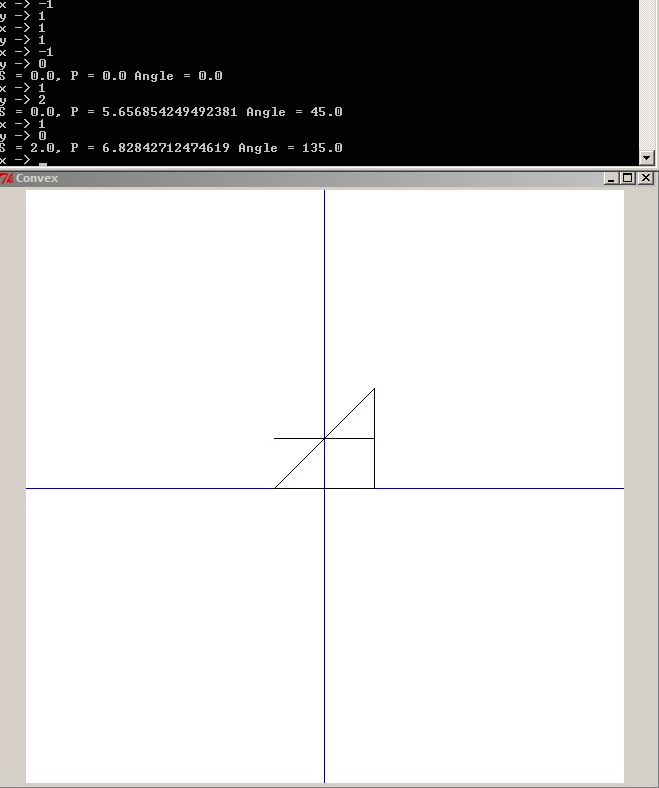
\includegraphics[width=0.8\hsize]{images/screen1}
\end{center}
\caption{Работа программы «Выпуклая оболочка»}
\end{figure}
\newpage











